\documentclass[tikz,border=10pt]{standalone}
\usetikzlibrary{positioning,arrows.meta}
\definecolor{eventFill}{HTML}{FFE0B2}
\definecolor{eventBorder}{HTML}{FB8C00}
\definecolor{subjectFill}{HTML}{C8E6C9}
\definecolor{subjectBorder}{HTML}{4CAF50}
\definecolor{observerFill}{HTML}{E1BEE7}
\definecolor{observerBorder}{HTML}{9C27B0}

\begin{document}
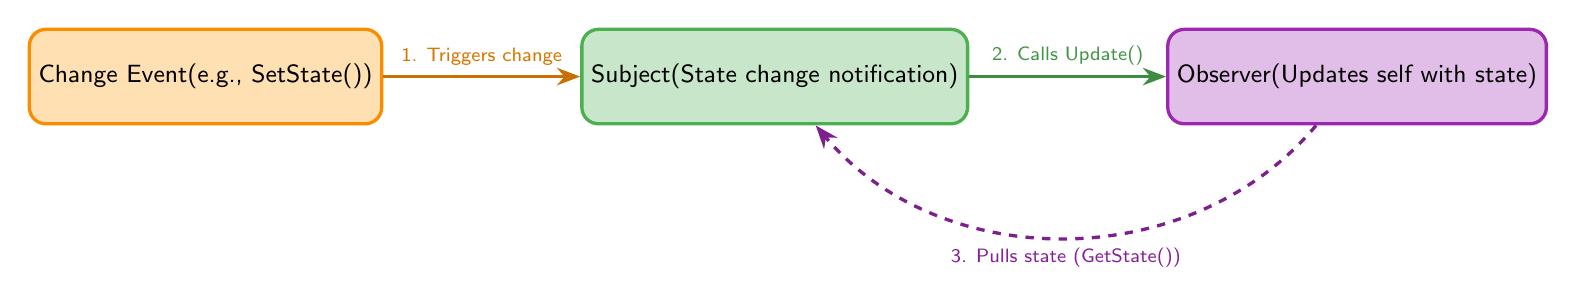
\begin{tikzpicture}[
    block/.style={
        rectangle, draw,
        minimum width=3.5cm, minimum height=1.2cm,
        text centered, rounded corners=6pt,
        line width=1.2pt, font=\sffamily\small
    },
    arrow/.style={-{Stealth[scale=1.0]}, line width=1.2pt}
]
  % Nodes
  \node[block, fill=eventFill, draw=eventBorder] (event) {Change Event\\(e.g., SetState())};
  \node[block, fill=subjectFill, draw=subjectBorder, right=2.5cm of event] (subject) {Subject\\(State change notification)};
  \node[block, fill=observerFill, draw=observerBorder, right=2.5cm of subject] (observer) {Observer\\(Updates self with state)};

  % Edges
  \draw[arrow, draw=eventBorder!80!black] (event) -- (subject) 
      node[midway, above, font=\sffamily\scriptsize, text=eventBorder!85!black] {1. Triggers change};
  
  \draw[arrow, draw=subjectBorder!80!black] (subject) -- (observer)
      node[midway, above, font=\sffamily\scriptsize, text=subjectBorder!85!black] {2. Calls Update()};
      
  % Backwards curved dashed arrow for pull - routed via bottom
  \draw[arrow, draw=observerBorder!80!black, dashed] (observer) to[out=230,in=310] 
      node[midway, below, font=\sffamily\scriptsize, text=observerBorder!85!black] {3. Pulls state (GetState())} (subject);

\end{tikzpicture}
\end{document}
